\documentclass[10pt, oneside]{article}
\usepackage{amsmath}
\usepackage{amssymb}
\usepackage[utf8]{inputenc}
\usepackage[english]{babel}
\usepackage{titling}
\usepackage[nottoc, notlof]{tocbibind}
\usepackage[pdftex]{graphicx}
\usepackage[kerning,spacing]{microtype}
\usepackage{verbatim}
\usepackage{tikz}
\usetikzlibrary{arrows}

\usepackage[bookmarksnumbered, unicode, pdftex]{hyperref}

\author{Mikhail Glushenkov, \texttt{<c05mgv@cs.umu.se>}\\
        Bertil Nilsson, \texttt{<id09bnn@cs.umu.se>}}

\title{Assignment 2 -- GCom Middleware:\\Analysis and Design}

\newcommand{\unit}[1]{\ensuremath{\, \mathrm{#1}}}

\begin{document}
\pagestyle{plain}
\pdfbookmark[1]{Front page}{beg}

\begin{titlingpage}
  \begin{minipage}[t]{0.45\textwidth}
  \begin{flushleft}
  \texttt{5DV020 - Distributed Systems, Autumn 12}
  \end{flushleft}
  \end{minipage}
  \begin{minipage}[t]{0.4\textwidth}
  \begin{flushright}
  \texttt{Umeå University}
  \end{flushright}
  \end{minipage}
  \vskip 60pt
  \begin{center}
  \LARGE\thetitle
  \par\end{center}\vskip 0.5em
  \begin{center}
  \large\theauthor
  \par\end{center}
  \begin{center}
  Date: \today
  \par\end{center}
  \vfill
  \begin{center}
    \textbf{Instructors} \linebreak \linebreak
    Francisco Hernandez-Rodriguez\\
    Ewnetu Bayuh Lakew
  \end{center}
\end{titlingpage}

% TOC
%\thispagestyle{empty}
%\pagebreak
%\setcounter{page}{0}
%\pdfbookmark[1]{Table of contents}{tab}
%\tableofcontents
\pagebreak

% % i Sverige har vi normalt inget indrag vid nytt stycke
\setlength{\parindent}{0pt}
% men däremot lite mellanrum
\setlength{\parskip}{10pt}

\setcounter{section}{-1}

\section{Introduction}

The purpose of this assignment is to design and implement GCom, a middleware for
group communication. Middleware is a software layer that provides a high-level
interface to some functionality and frees the user from worrying about how said
functionality is implemented. Group communication is a mode of communication
that allows a set of nodes distributed over network to form groups and broadcast
messages to all members of the groups they belong to.

This is the first report, written at the planning stage of the project. It
contains a requirements specification, a description of the design and a time
plan.

\section{Requirements Specification}

This assignment is divided into three levels - the obligatory basic level and
two bonus levels that give additional points. In addition to the basic level,
our solution will also implement the first bonus level (dynamic groups).

The GCom middleware consists of three logical modules: communication, message
ordering and group management. Additionally, we are required to implement a GUI
test application for showcasing the features of the GCom middleware and a GUI
debug application for demonstrating that it works correctly.

The communication module supports two operations: basic non-reliable multicast
and basic reliable multicast. The type of multicast and the message type are set
at module initialisation time, so only a single send operation is accessible at
runtime. This operation takes a set of nodes and a message as input, and blocks
until the operation has completed. The communication module also allows to
register callbacks for acting upon a message delivired to the current node.

The message ordering module is built on top of the communication module. It
allows to deliver messages according to several different orderings. The
following orderings must be supported: non-ordered, FIFO, causal, total and
causal-total (described in more detail in the assignment specification and in
the textbook\cite{Textbook}). Again, the type of ordering is set at module
initialisation time. Apart from this, this module has the same interface as the
communication module, if we don't take support for the debugging application
into account.

The group management module is the user-facing part of the system implemented on
top of the previous two modules. It allows to create and remove groups, add and
remove group members, handles the monitoring of live nodes, keeps track of
changes in group membership, and allows to list the names of all existing
groups.

The test program is a simple distributed GUI chat program in which each chat
client instance is a node of the distributed system.

The debug application is implemented as a special client for the aforementioned
chat system that allows to watch the inner workings of the middleware. It has
the following features:
\begin{itemize}
\item Simulated packet loss (send a message to a part of the group).
\item Simulated packet rearrangement (send several messages in random order to
  different nodes).
\item Simulated packet delay (broadcast a message, but delay dispatching to some
  nodes).
\item Creation of a group with a chosen message ordering and multicast type.
\item Display of the internal state of the system (such as message queues).
\item Measurement of system performance.
\end{itemize}

\section{Design}

We decided to implement our system in Scala and use Java RMI for communication
between nodes. The choice of Scala was motivated by the desire to use a language
that is more modern and convenient than Java, but still allows to run on
JVM. Java RMI was chosen because it was the default option (recommended in the
assignment specification) and we felt that other messaging solutions that we
looked at either didn't provide any benefit for our use case (Finagle) or did
all the required work for us (ZeroMQ).

The communication module is just a straightforward implementation of the
textbook algorithms for reliable and unreliable multicast\cite{Textbook}. The
same can be said about the message ordering module: FIFO ordering will be
implemented with logical timestamps, vector clocks will be used for the causal
ordering, total ordering will be implemented with a sequencer node (specified as
one of the inputs to the send function), and causal-total is just a combination
of causal and total.

\begin{figure}[h]
\centering
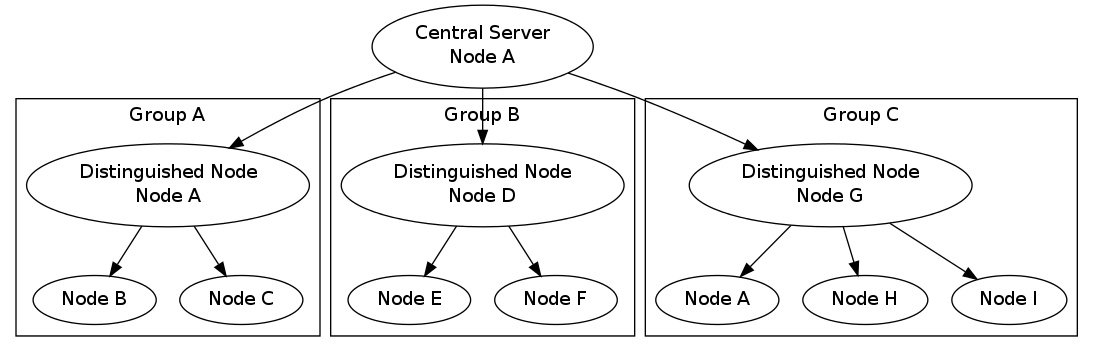
\includegraphics[width=12cm]{graph1}
\caption{Group management module.}
\label{fig:group}
\end{figure}

The group management module has a slightly more complicated design. Each node is
identified by a (host, port number, name) triple. A group is identified by its
name; names are globally unique, which is enforced by a central server that also
associates an ID of a coordinator node with each group name. The central server
is used a hub through each new nodes can discover and join existing groups.

The coordinator node in each group serves as a message sequencer and gateway
through which new nodes join the group. The process of joining a group is
illustrated in figure~\ref{fig:group}. A node first contacts the central server,
which knows the names of all groups and all coordinator nodes. When a node has
chosen which group it wants to join, it contacts the coordinator for that group
and receives the list of all group members. The group members then synchronise
its view of group membership and the node is considered admitted.

If the coordinator node dies or leaves the group, a new coordinator is elected,
and all group members and the central server are notified. The Paxos
algorithm\cite{Paxos} is used to ensure that all nodes have a consistent view of
group membership, group coordinator and the value of the total ordering
counter. The choice of Paxos was motivated by it being used for similar purposes
in such real-world systems as Google Chubby\cite{Chubby}, IBM
Spinnaker\cite{Spinnaker} and Doozer\cite{Doozer}.

In case a group gets partitioned, each partition will elect a new coordinator
and will continue to function independently. The ones that can't contact the
central server will know that they are the ones ``left behind''. They can choose
to either shut down, continue to communicate among themselves or wait for the
central server to become available and try to rejoin the group.

The system is designed to scale fairly well, since at no point there is a need
to communicate with or store the names of all nodes in the system. Each node
communicates only with the members of the groups it belongs to, and the central
server communicates only with the coordinator nodes. The central server is
obviously a single point of failure, but the groups don't depend on it to
function and we believe that a central group catalog is needed in any case so
that new nodes can discover what groups exist in the system.

We expect our system to be able to support large numbers of groups and
nodes. The exact limits will be determined empirically.

\pagebreak

\section{Time Plan}

Our preliminary plan looks as follows:

\begin{tabular}{|l|p{10cm}|}
  \hline
  Week 49 & Implement the communication module. Start working on implementing the
  Paxos algorithm. Start working on the GUI test programs. \\
  \hline
  Week 50 & Implement the message ordering module. Produce a finished version of the Paxos algorithm. \\
  \hline
  Week 51 & Integrate the code written during the first two weeks; produce an
  initial approximation of the final system. \\
  \hline
  Week 52 & Testing and bugfixing. Work on the test programs. Start writing the final report. \\
  \hline
  Week 1  & More testing and bugfixing. Time for any unforeseen delays. \\
  \hline
  Week 2  & Practical demonstration. Turn in the final report. \\
  \hline
\end{tabular}

\begin{thebibliography}{9}

\bibitem{Textbook} \emph{Distributed Systems}\\
\newblock George Coulouris, Jean Dollimore, Tim Kindberg and Gordon Blair\\
\newblock Addison-Wesley, 2011\\

\bibitem{Paxos} \emph{Paxos Made Simple}\\
\newblock Leslie Lamport\\
\newblock ACM SIGACT News (Distributed Computing Column) 32, 4 (Whole Number
121, December 2001) 51-58.\\

\bibitem{Chubby} \emph{The Chubby Lock Service for Loosely-Coupled Distributed}\\
\newblock Mike Burrows\\
\newblock OSDI'06: Seventh Symposium on Operating System Design and Implementation,
Seattle, WA, November, 2006.\\
\newblock \url{http://research.google.com/archive/chubby.html}\\
\newblock URL accessed \today\\

\bibitem{Doozer} \emph{Doozer -- a highly-available, completely consistent store for
    small amounts of extremely important data.}\\
\newblock Blake Mizerany, Keith Rarick et al.\\
\newblock \url{https://github.com/ha/doozerd} \\
\newblock URL accessed \today\\

\bibitem{Spinnaker} \emph{Using Paxos to Build a Scalable, Consistent, and
    Highly Available Datastore}\\
\newblock Jun Rao, Eugene J. Shekita, Sandeep Tata\\
\newblock Proceedings of the VLDB Endowment (PVLDB), Vol. 4, No. 4, pp. 243-254
(2011)\\
\newblock \url{http://arxiv.org/abs/1103.2408}\\
\newblock URL accessed \today\\

\end{thebibliography}


\end{document}
